\documentclass{beamer}
% \documentclass{article}
% \usepackage{beamerarticle}

\usepackage{mathtools}
\usepackage{stmaryrd}
\usepackage{tikz}
\usetikzlibrary{arrows.meta,arrows}
\usetikzlibrary{positioning}

\usetheme{Boadilla}
\setbeamercovered{transparent} 
\usefonttheme[onlymath]{serif}

\newcommand{\While}{\textbf{While}}
\newcommand{\ExtWhile}{\textbf{While}\ensuremath{^{\mbox{\footnotesize ext}}}}
\newcommand{\Num}{\textbf{Num}}
\newcommand{\Var}{\textbf{Var}}
\newcommand{\Aexp}{\textbf{Aexp}}
\newcommand{\Bexp}{\textbf{Bexp}}
\newcommand{\Stm}{\textbf{Stm}}
\newcommand{\State}{\textbf{State}}
\newcommand{\Z}{\mathbb{Z}}
\newcommand{\T}{\textbf{T}}
\newcommand{\true}{\texttt{true}}
\newcommand{\false}{\texttt{false}}
\newcommand{\sskip}{\texttt{skip}}
\newcommand{\ifelse}[3]{\mathtt{if}\ #1\ \mathtt{then}\ #2\ \mathtt{else}\ #3\ \mathtt{endif}}
\newcommand{\while}[2]{\mathtt{while}\ #1\ \mathtt{do}\ #2\ \mathtt{done}}
\newcommand{\sem}[2]{\mathcal{#1} \llbracket #2 \rrbracket}
\newcommand{\tr}{\mathbf{tt}}
\newcommand{\ff}{\mathbf{ff}}
\newcommand{\undefined}{\uparrow}
\newcommand{\defined}{\!\downarrow}

\newcommand{\Intmn}{\textrm{I}_{\textrm{m,n}}}
\newcommand{\bound}{\textrm{bound}_{\textrm{m,n}}}

\title{Implementation of Abstract Interpreter}
\subtitle{Software Verification Course Homework}
\author[E. Scandaletti]{Elia Scandaletti\texorpdfstring{ - 2087934\\University of Padova}{}}
\date[13/02/2023]{16th March 2023}

\begin{document}
\begin{frame}
    \titlepage
\end{frame}

\begin{frame}{Outline}
    \tableofcontents
\end{frame}

\section{Program Overview}

\begin{frame}{Program Overview}

    The program is composed of three main parts:

    \begin{block}{Parsing}
        The syntax module provides the function \texttt{build\_ast} that transform the input into an Abstract Syntax Tree.
    \end{block}

    \begin{block}{Building the Control Flow Graph}
        The Abstract Syntax Tree is then transformed in a Control Flow Graph via the \texttt{new} constructor.
    \end{block}

    \begin{block}{Abstract Execution}
        The program is abstractly executed on the control flow graph.
    \end{block}

    ~\\
    We will see each of them in detail.

\end{frame}

\section{Extended While Language}

\begin{frame}{Extended While Syntax}

    \begin{align*}
        \mbox{\Aexp: }
        a \Coloneq    & \ n
        \ |\ x
        \ |\ a_1 + a_2
        \ |\ a_1 * a_2
        \ |\ a_1 - a_2                     \\
        \ |\          & a_1 \div a_2
        \ |\ x+\!+
        \ |\ +\!+x
        \ |\ x-\!-
        \ |\ -\!-x
        \\
        \mbox{\Bexp: }
        b \Coloneq    & \ \true
        \ |\ \false
        \ |\ \neg b
        \ |\ b_1 \wedge b_2
        \ |\ a_1 = a_2
        \ |\ a_1 \leq a_2
        \\
        \mbox{\Stm: }
        S \Coloneq    & \ x \coloneq a
        \ |\ \sskip
        \ |\ S_1; S_2
        \ |\ \ifelse{b}{S_1}{S_2}          \\
        \ |\          & \while{b}{S}
        \ |\ a
        \ |\ b
        \ |\ \alert{[spec]} S
        \\
        spec \Coloneq & \ \mathtt{w}\ spec
        \ |\ \mathtt{n}\ spec
    \end{align*}

    $n \in \mathbf{Num}$ is a string of decimal digits.

    $x \in \mathbf{Var}$ is a string of alphabetical ASCII characters.

    ~\\
    $[spec]$ is used to specify the set of points used for widening or narrowing.

\end{frame}

\begin{frame}{Extended While Concrete Semantics}{State Changing Arithmetic Expressions}

    $$\mathcal{S_A} : \Aexp \to \State \to \State$$
    \begin{gather*}
        \begin{aligned}
            \sem{S_A}{n}      & = \mathrm{id}         &
            \sem{S_A}{x}      & = \mathrm{id}           \\
            \sem{S_A}{x+\!+}s & = s[x \mapsto s\;x+1] &
            \sem{S_A}{x-\!-}s & = s[x \mapsto s\;x-1]   \\
            \sem{S_A}{+\!+x}s & = s[x \mapsto s\;x+1] &
            \sem{S_A}{-\!-x}s & = s[x \mapsto s\;x-1]   \\
        \end{aligned} \\
        \begin{aligned}
            \forall \star \in \{+, -, *, \div\}\
            \sem{S_A}{a_1 \star a_2} & = \sem{S_A}{a_2} \circ \sem{S_A}{a_1}
        \end{aligned}
    \end{gather*}

\end{frame}

\begin{frame}{Extended While Concrete Semantics}{Value of Arithmetic expressions}

    $$\mathcal{V_A} : \Aexp \to \State \hookrightarrow \Z$$
    \begin{gather*}
        \begin{aligned}
            \sem{V_A}{n}s     & = \sem{N}{n} &
            \sem{V_A}{x}s     & = s\;x         \\
            \sem{V_A}{x+\!+}s & = s\;x       &
            \sem{V_A}{x-\!-}s & = s\;x         \\
            \sem{V_A}{+\!+x}s & = s\;x+1     &
            \sem{V_A}{-\!-x}s & = s\;x-1
        \end{aligned} \\
        \begin{aligned}
            \sem{V_A}{a_1 \star a_2}s & =
            \begin{cases}
                z_1 \star z_2,
                 & \mbox{if } \sem{V_A}{a_1}s \defined = z_1 \wedge \sem{S_A}{a_1}s = s' \\
                 & \wedge \sem{V_A}{a_2}s' \defined = z_2                                \\
                \undefined,
                 & \mbox{otherwise}
            \end{cases} \\
            \sem{V_A}{a_1 \div a_2}s  & =
            \begin{cases}
                z_1 \div z_2,
                 & \mbox{if } \sem{V_A}{a_1}s \defined = z_1 \wedge \sem{S_A}{a_1}s = s' \\
                 & \wedge \sem{V_A}{a_2}s' \defined = z_2 \neq 0                         \\
                \undefined,
                 & \mbox{otherwise}
            \end{cases}
        \end{aligned}
    \end{gather*}

\end{frame}

\begin{frame}{Extended While Concrete Semantics}{State Changing Boolean Expressions}

    $$\mathcal{S_B} : \Bexp \to \State \to \State$$
    \begin{align*}
        \sem{S_B}{\true}          & = \mathrm{id}                         \\
        \sem{S_B}{\false}         & = \mathrm{id}                         \\
        \sem{S_B}{\neg b}         & = \sem{S_B}{b}                        \\
        \sem{S_B}{b_1 \wedge b_2} & = \sem{S_B}{b_2} \circ \sem{S_B}{b_1} \\
        \sem{S_B}{a_1 = a_2}      & = \sem{S_A}{a_2} \circ \sem{S_A}{a_1} \\
        \sem{S_B}{a_1 \leq a_2}   & = \sem{S_A}{a_2} \circ \sem{S_A}{a_1}
    \end{align*}

\end{frame}

\begin{frame}{Extended While Concrete Semantics}{Value of Boolean Expressions}

    $$\mathcal{V_B} : \Bexp \to \State \hookrightarrow \T$$
    \begin{overprint}
        \onslide<1>
        \begin{gather*}
            \begin{aligned}
                \sem{V_B}{\true}s  & = \tr &
                \sem{V_B}{\false}s & = \ff   \\
            \end{aligned} \\
            \sem{V_B}{\neg b}s =
            \begin{cases}
                \tr,        & \mbox{if } \sem{V_B}{b}s \defined = \ff \\
                \ff,        & \mbox{if } \sem{V_B}{b}s \defined = \tr \\
                \undefined, & \mbox{otherwise}
            \end{cases}
        \end{gather*}

        \onslide<2>
        \begin{equation*}
            \sem{V_B}{b_1 \wedge b_2}s =
            \begin{cases}
                \tr,
                 & \mbox{if } s' = \sem{S_B}{b_1}s \;\wedge                   \\
                 & \sem{V_B}{b_1}s \defined = \sem{V_B}{b_2}s' \defined = \tr \\
                \ff,
                 & \mbox{else if } s' = \sem{S_B}{b_1}s \;\wedge              \\
                 & \sem{V_B}{b_1}s \defined \wedge \sem{V_B}{b_2}s' \defined  \\
                \undefined,
                 & \mbox{otherwise}
            \end{cases}
        \end{equation*}

        \onslide<3>
        \begin{equation*}
            \sem{V_B}{a_1 = a_2}s =
            \begin{cases}
                \tr,
                 & \mbox{if } s' = \sem{S_A}{a_1}s \;\wedge                  \\
                 & \sem{V_A}{a_1}s \defined \;= \sem{V_A}{a_2}s' \defined    \\
                \ff,
                 & \mbox{else if } s' = \sem{S_A}{a_1}s \;\wedge             \\
                 & \sem{V_A}{a_1}s \defined \wedge \sem{V_A}{a_2}s' \defined \\
                \undefined,
                 & \mbox{otherwise}
            \end{cases}
        \end{equation*}

        \onslide<4>
        \begin{equation*}
            \sem{V_B}{a_1 \leq a_2}s =
            \begin{cases}
                \tr,
                 & \mbox{if } s' = \sem{S_A}{a_1}s \;\wedge                  \\
                 & \sem{V_A}{a_1}s \defined \;\leq \sem{V_A}{a_2}s' \defined \\
                \ff,
                 & \mbox{else if } s' = \sem{S_A}{a_1}s \;\wedge             \\
                 & \sem{V_A}{a_1}s \defined \wedge \sem{V_A}{a_2}s' \defined \\
                \undefined,
                 & \mbox{otherwise}
            \end{cases}
        \end{equation*}
    \end{overprint}

\end{frame}

\begin{frame}{Denotational Semantics}{Semantic Function}

    $$\mathcal{S}_{\mathrm{ds}}: \Stm \to \State \hookrightarrow \State$$
    \begin{overprint}
        \onslide<1>
        \begin{align*}
            \sem{S_{\mathrm{ds}}}{x \coloneq a}s & =
            (\mathrm{set}(x, \sem{V_A}{a}s) \circ \sem{S_\mathrm{ds}}{a})s \\
            \mbox{where } \mathrm{set}(x, z)\;s  & =
            \begin{cases}
                s[x \mapsto z], & \mbox{if } z\defined \\
                \undefined,     & \mbox{otherwise}
            \end{cases}                         \\
            \sem{S_{\mathrm{ds}}}{\sskip}        & =
            \mathrm{id}                                                    \\
            \sem{S_{\mathrm{ds}}}{S_1; S_2}      & =
            \sem{S_{\mathrm{ds}}}{S_2} \circ \sem{S_{\mathrm{ds}}}{S_1}    \\
            \sem{S_{\mathrm{ds}}}{a}             & =
            \sem{S_A}{a}                                                   \\
            \sem{S_{\mathrm{ds}}}{b}             & =
            \sem{S_B}{b}
        \end{align*}

        \onslide<2>
        \begin{gather*}
            \begin{multlined}[][0.8\textwidth]
                \sem{S_{\mathrm{ds}}}{\ifelse{b}{S_1}{S_2}} = \\
                \mathrm{cond}(\sem{V_B}{b}, \sem{S_\mathrm{ds}}{b}, \sem{S_{\mathrm{ds}}}{S_1}, \sem{S_{\mathrm{ds}}}{S_2})
            \end{multlined} \\
            \mbox{where } \mathrm{cond}(p, g_0, g_1, g_2)\;s =
            \begin{cases}
                g_1\;(g_0\;s), & \mbox{if } p\;s\defined = \tr \\
                g_2\;(g_0\;s), & \mbox{if } p\;s\defined = \ff \\
                \bot,          & \mbox{otherwise}
            \end{cases}
        \end{gather*}
        Note that the functionality of $\mathrm{cond}$ is:
        \begin{multline*}
            (\State \hookrightarrow \T) \times (\State \hookrightarrow \State) \times \\
            (\State \hookrightarrow \State) \times (\State \hookrightarrow \State) \to (\State \hookrightarrow \State)
        \end{multline*}

        \onslide<3>
        \begin{align*}
            \sem{S_{\mathrm{ds}}}{\while{b}{S}} & =
            \mathrm{FIX}\;F                         \\
            \mbox{where } F\;g                  & =
            \mathrm{cond}(\sem{V_B}{b}, \sem{S_\mathrm{ds}}{b}, g \circ \sem{S_{\mathrm{ds}}}{S},\mathrm{id})
        \end{align*}

        This comes from the semantic equivalence
        \begin{multline*}
            \sem{S_{\mathrm{ds}}}{\while{b}{S}} \\
            = \sem{S_{\mathrm{ds}}}{\ifelse{b}{(S; \while{b}{S})}{\sskip}} \\
            = \mathrm{cond}(\sem{V_B}{b}, \sem{S_\mathrm{ds}}{b}, \sem{S_{\mathrm{ds}}}{S; \while{b}{S}},\mathrm{id}) \\
            = \mathrm{cond}(\sem{V_B}{b}, \sem{S_\mathrm{ds}}{b}, \sem{S_{\mathrm{ds}}}{\while{b}{S}} \circ \sem{S_{\mathrm{ds}}}{S},\mathrm{id})
        \end{multline*}
    \end{overprint}

\end{frame}

\section{Parsing}

\begin{frame}{Pest crate}

    The Rust crate \texttt{pest} provides a way of defining a parsing expression grammar which is then used to provide a stream of tokens given an input.

    ~\\
    The stream can be mapped recursively thanks to an utility of the same crate: the \texttt{pratt\_parser}.

    This parser arranges the tokens hierarchically in a n-ary tree.
    The number of children of a node depends on the rule corresponding to the node.
    Therefore, it's easy to convert this structure in an Abstract Syntax Tree.

\end{frame}

\begin{frame}{Abstract Syntax Tree}

    The Abstract Syntax Tree represents the structure of the input program.
    It has three types of components:
    \begin{itemize}
        \item \texttt{AExp}: represents an arithmetic expression;
        \item \texttt{BExp}: represents a boolean expression;
        \item \texttt{Stm}: represents a statement.
    \end{itemize}

    ~\\
    Each of these types is implemented as an enum.

\end{frame}

\begin{frame}{Abstract Syntax Tree}{\texttt{AExp}}

    Arithmetic expressions have multiple variants:
    \begin{itemize}
        \item \texttt{Num(\textit{n})} $\sim$ \texttt{\textit{n}};
        \item \texttt{Var(\textit{x})} $\sim$ \texttt{\textit{x}},
        \item \texttt{Add(\textit{a1}, \textit{a2})} $\sim$ \texttt{\textit{a1} + \textit{a2}};
        \item \texttt{Sub(\textit{a1}, \textit{a2})} $\sim$ \texttt{\textit{a1} - \textit{a2}};
        \item \texttt{Mul(\textit{a1}, \textit{a2})} $\sim$ \texttt{\textit{a1} * \textit{a2}};
        \item \texttt{Div(\textit{a1}, \textit{a2})} $\sim$ \texttt{\textit{a1} / \textit{a2}};
        \item \texttt{Neg(\textit{a})} $\sim$ \texttt{-\textit{a}};
        \item \texttt{PreInc(\textit{x})} $\sim$ \texttt{++\textit{x}};
        \item \texttt{PreDec(\textit{x})} $\sim$ \texttt{--\textit{x}};
        \item \texttt{PostInc(\textit{x})} $\sim$ \texttt{\textit{x}++};
        \item \texttt{PostDec(\textit{x})} $\sim$ \texttt{\textit{x}--}.
    \end{itemize}

\end{frame}

\begin{frame}{Abstract Syntax Tree}{\texttt{BExp}}

    Boolean expressions have multiple variants:
    \begin{itemize}
        \item \texttt{True} $\sim$ \texttt{true};
        \item \texttt{False} $\sim$ \texttt{false};
        \item \texttt{Eq(\textit{a1}, \textit{a2})} $\sim$ \texttt{\textit{a1} = \textit{a2}};
        \item \texttt{Neq(\textit{a1}, \textit{a2})} $\sim$ \texttt{\textit{a1} != \textit{a2}};
        \item \texttt{Lt(\textit{a1}, \textit{a2})} $\sim$ \texttt{\textit{a1} < \textit{a2}};
        \item \texttt{And(\textit{b1}, \textit{b2})} $\sim$ \texttt{\textit{b1} \&\& \textit{b2}};
        \item \texttt{Or(\textit{b1}, \textit{b2})} $\sim$ \texttt{\textit{b1} || \textit{b2}};
        \item \texttt{Not(\textit{b})} $\sim$ \texttt{!\textit{b}}.
    \end{itemize}

\end{frame}

\begin{frame}{Abstract Syntax Tree}{\texttt{Stm}}

    Statements have multiple variants:
    \begin{itemize}
        \item \texttt{AExp(meta, \textit{a})} $\sim$ \textit{a}, result is ignored;
        \item \texttt{BExp(meta, \textit{b})} $\sim$ \textit{b}, result is ignored;
        \item \texttt{Ass(meta, \textit{x}, \textit{a})} $\sim$ \texttt{\textit{x} := \textit{a}};
        \item \texttt{Skip(meta)} $\sim$ \sskip;
        \item \texttt{IfThenElse(meta, \textit{b}, \textit{stm1}, \textit{stm2})} $\sim$ \\
              \hskip 1.5cm \texttt{if \textit{b} then \textit{stm1} else \textit{stm2} endif};
        \item \texttt{While(meta, \textit{b}, \textit{stm})} $\sim$ \texttt{while \textit{b} do \textit{stm} done};
        \item \texttt{Comp(\textit{stm1}, \textit{stm2})} $\sim$ \texttt{\textit{stm1}; \textit{stm}2}.
    \end{itemize}

    ~\\
    Note that all the statements - except \texttt{Comp} - have a \texttt{meta} field which contains some useful information: the label of the node just before the statement and whether it is a widening and/or narrowing point.

\end{frame}

\section{Building the Control Flow Graph}

\begin{frame}{Control Flow Graph}

    The Control Flow Graph is a graph in which each vertex represents a point of a program.

    Each arc, instead, represents a command.
    A command can be either a statement or a boolean guard.

    \begin{itemize}
        \item \texttt{Guard(\textit{b})}: represents the states for which \textit{b} evaluated to true;
        \item \texttt{AExp(\textit{a})}, \texttt{BExp(\textit{b})}, \texttt{Ass(\textit{x}, \textit{a})}, \texttt{Skip}: represent how the corresponding statements modify the state.
    \end{itemize}

    ~\\
    Note that the \texttt{While}, \texttt{IfThenElse} and \texttt{Comp} do not appear.
    This kinds of statement are used to build the structure of the graph.
    Their boolean guards and sub-statements become arcs of the graph.

\end{frame}

\begin{frame}{Control Flow Graph}{IfThenElse}

    \texttt{if \textit{b} then \textit{stm1} else \textit{stm2} endif}

    ~\\~\\\centering
    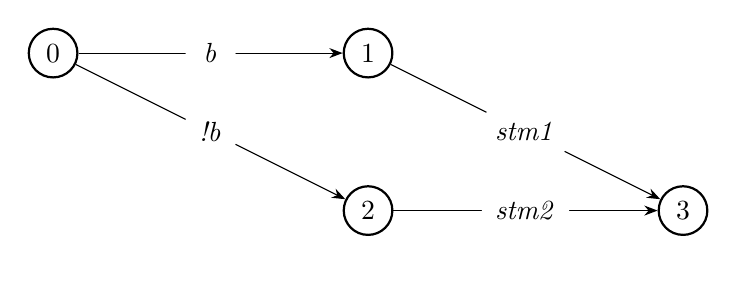
\begin{tikzpicture}

        \begin{scope}[every node/.style={circle,thick,draw}]
            \node (A) at (1,3) {0};
            \node (B) at (5,3) {1};
            \node (C) at (5,1) {2};
            \node (D) at (9,1) {3};
        \end{scope}

        \begin{scope}[>={Stealth[black]},
            every node/.style={fill=white,circle}]
            \path [->] (A) edge node {\textit{b}} (B);
            \path [->] (A) edge node {\textit{!b}} (C);
            \path [->] (B) edge node {\textit{stm1}} (D);
            \path [->] (C) edge node {\textit{stm2}} (D);
        \end{scope}
    \end{tikzpicture}

\end{frame}

\begin{frame}{Control Flow Graph}{While}

    \texttt{while \textit{b} do \textit{stm} done}

    ~\\~\\\centering
    \begin{tikzpicture}

        \begin{scope}[every node/.style={circle,thick,draw}]
            \node (A) at (3,5) {0};
            \node (B) at (1,1) {1};
            \node (C) at (7,3) {2};
        \end{scope}

        \begin{scope}[>={Stealth[black]},
            every node/.style={fill=white,circle}]
            \path [->] (A) edge[bend right=30] node {\textit{b}} (B);
            \path [->] (A) edge node {\textit{!b}} (C);
            \path [->] (B) edge[bend right=30] node {\textit{stm}} (A);
        \end{scope}
    \end{tikzpicture}

\end{frame}

\begin{frame}{Control Flow Graph}{Comp}

    \texttt{\textit{stm1}; \textit{stm2}}

    ~\\~\\\centering
    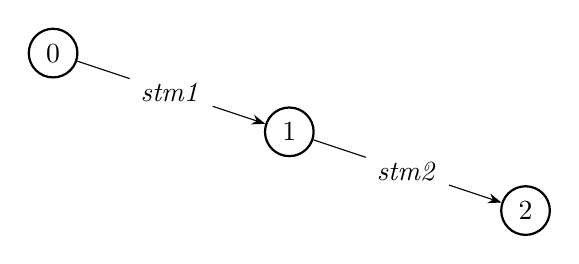
\begin{tikzpicture}

        \begin{scope}[every node/.style={circle,thick,draw}]
            \node (A) at (1,3) {0};
            \node (B) at (4,2) {1};
            \node (C) at (7,1) {2};
        \end{scope}

        \begin{scope}[>={Stealth[black]},
            every node/.style={fill=white,circle}]
            \path [->] (A) edge node {\textit{stm1}} (B);
            \path [->] (B) edge node {\textit{stm2}} (C);
        \end{scope}
    \end{tikzpicture}

\end{frame}

\section{Abstract Value Domain}

\begin{frame}{Abstract Value Domain}

    Trait \texttt{AbsValueDomain} requires:
    \begin{itemize}
        \item associated type \texttt{Value};
        \item method \texttt{value\_from\_num} to convert a numeral into a \texttt{Value};
        \item method \texttt{cmp} to compare \texttt{Value}s;
        \item methods \texttt{neg}, \texttt{add}, \texttt{sub}, \texttt{mul} and \texttt{div} to perform arithmetic operations on \texttt{Value}s;
        \item methods \texttt{top} and \texttt{bot} which return the top and bottom elements of the domain;
        \item methods \texttt{lub} and \texttt{glb} to perform the corresponding operations;
        \item methods \texttt{widening} and \texttt{narrowing} to perform the corresponding operations.
    \end{itemize}

\end{frame}

\begin{frame}{Interval Domain}

    \begin{overprint}
        \onslide<1>
        \begin{block}{\texttt{Value}}
            \begin{multline*}
                \Intmn = \{ \emptyset, \mathbb{Z} \}
                \cup \{ [a, b]\, |\, [a, b] \subseteq [m, n] \}
                \cup \{ [k, k]\, |\, k \in \mathbb{Z} \} \\
                \cup \{ (-\inf, k]\, |\, k \in [m, n] \}
                \cup \{ [k, +\inf)\, |\, k \in [m, n] \}
            \end{multline*}
            The empty element is represented as the special value \texttt{Bot}.

            $\mathbb{Z}$ is represented as the interval $(-\inf, +\inf)$.
        \end{block}

        \onslide<2>
        \begin{block}{Conversion from interval}
            $$\bound : \cal{B}^\# \to \Intmn $$
            $$
                \bound\ [a,b] =
                \begin{cases}
                    \bot^\#_{\Intmn}, & \mbox{if } a > b                 \\
                    \top^\#_{\Intmn}, & \mbox{if } a < m \wedge b > n    \\
                    [a, b],           & \mbox{if } a = b                 \\
                    [-\inf, b],       & \mbox{if } a < m \wedge b \leq n \\
                    [a, +\inf],       & \mbox{if } b > n \wedge a \geq m
                \end{cases}
            $$
        \end{block}

        \onslide<3>
        \begin{block}{POSet operators}
            $$
                [a,b] \sqsubseteq_{\Intmn} [c,d] \iff a \geq c \wedge b \leq d
            $$
            $$
                \top^\#_{\Intmn} = \left] \textrm{-inf}, \textrm{+inf} \right[
            $$
            $$
                [a,b] \cup^\#_{\Intmn} [c,d] = \bound\ [\min(a,c), \max(b,d)]
            $$
            $$
                [a,b] \cap^\#_{\Intmn} [c,d] = \bound\ [\max(a,c), \min(b,d)]
            $$
        \end{block}

        \onslide<4>
        \begin{block}{Arithmetic operators}
            \begin{align*}
                -^\#_{\Intmn}[a,b]        & = \bound\ [-b, -a]   \\
                [a,b] +^\#_{\Intmn} [c,d] & = \bound\ [a+c,b+d]  \\
                [a,b] -^\#_{\Intmn} [c,d] & = \bound\ [a-d, b-c] \\
            \end{align*}
            \vspace{-3em}
            \begin{gather*}
                [a,b] \times^\#_{\Intmn} [c,d] = \bound\ \min(ac, ad, bc, bd), \max(ac, ad, bc, bd)] \\
                [a,b] /^\#_{\Intmn} [c,d] = \bound\
                \begin{cases}
                    [\min(a/c, a/d), \max(b/c, b/d)], \mbox{if } 1 \leq c  \\
                    [\min(b/c, b/d), \max(a/c, a/d)], \mbox{if } d \leq -1 \\
                    \begin{gathered}
                        ([a,b] /^\#_{\Intmn} ([c,d] \cap^\#_{\Intmn} [1,+\inf])) \\
                        \cup^\#_{\Intmn} \\
                        ([a,b] /^\#_{\Intmn} ([c,d] \cap^\#_{\Intmn} [-\inf,-1]))
                    \end{gathered}, \mbox{otherwise}
                \end{cases}
            \end{gather*}
        \end{block}

        \onslide<5>
        \begin{block}{Widening}
            $$
                \bot^\#_{\Intmn} \nabla_{\Intmn} X^\# = X^\#
            $$
            $$
                [a,b]\ \nabla_{\Intmn}\ [c,d] = \bound\ \left[
                    \begin{cases}
                        a,     & \mbox{if } a \leq c \\
                        -\inf, & \mbox{otherwise}
                    \end{cases},
                    \begin{cases}
                        b,     & \mbox{if } b \geq d \\
                        +\inf, & \mbox{otherwise}
                    \end{cases}
                    \right]
            $$
        \end{block}
        \begin{block}{Narrowing}
            $$
                [a,b]\ \Delta_{\Intmn}\ [c,d] = \bound\ \left[
                    \begin{cases}
                        c, & \mbox{if } a = -\inf \\
                        a, & \mbox{otherwise}
                    \end{cases},
                    \begin{cases}
                        d, & \mbox{if } b = +\inf \\
                        b, & \mbox{otherwise}
                    \end{cases}
                    \right]
            $$
        \end{block}
    \end{overprint}

\end{frame}

\section{Abstract State Domain}

\begin{frame}{Abstract State Domain}

    Trait \texttt{AbsDomain<AVD>} requires:
    \begin{itemize}
        \item the type parameter \texttt{AVD} must satisfy the \texttt{AbsValueDomain} trait;
        \item associated type \texttt{State};
        \item method \texttt{value\_domain} returning a copy of the abstract value domain used;
        \item methods \texttt{ass} and \texttt{get\_var} to assign and retrieve the abstract value of a variable in a given state;
        \item methods \texttt{bot}, \texttt{top} to get the bottom and the top elements of the domain;
        \item methods \texttt{lub}, \texttt{glb}, \texttt{widening} and \texttt{narrowing} to perform the respective operations.
    \end{itemize}

\end{frame}

\begin{frame}{Non Relational Domain}

    The \texttt{NonRelationalDomain<AVD>} structure implements the \texttt{AbsDomain<AVD>} trait.
    \begin{itemize}
        \item type \texttt{State} is either a special value \texttt{Bot} or a \texttt{Variable} to \texttt{AVD::Value} map;
              \begin{itemize}
                  \item invariant of \texttt{State}: if a stored variable has value bottom, the whole state becomes \texttt{Bot};
              \end{itemize}
        \item method \texttt{value\_domain} returns a copy of the abstract value domain stored in a private field;
        \item methods \texttt{ass} and \texttt{get\_var} write to and read from the given state;
        \item methods \texttt{bot} returns a state with vale \texttt{Bot};
        \item \texttt{top} returns a state with a map where all stored variables have value top;
        \item \texttt{lub}, \texttt{glb}, \texttt{widening} and \texttt{narrowing} are performed variable wise.
    \end{itemize}

\end{frame}

\section{Abstracting the Execution}

\begin{frame}{Abstract Execution}{Arithmetic Expressions}

    Arithmetic expressions are evaluated recursively in postfix order.

    Each evaluation has two outputs:
    \begin{itemize}
        \item the state modified by the execution;
        \item the result of the expression.
    \end{itemize}

    In the implementation, the first one is a mutable reference passed as argument.
    The second one, is the value returned by the function.

\end{frame}

\begin{frame}{Abstract Execution}{Boolean Expressions}

    Boolean expressions are evaluated recursively in postfix order.

    Each evaluation has two outputs:
    \begin{itemize}
        \item how the state is modified by the execution;
        \item the result of the expression, represented as the set of states for which the expression is true.
    \end{itemize}

    In the implementation, the first one is a mutable reference passed as argument.
    The second one, is the value returned by the function.

\end{frame}

\begin{frame}{Abstract Execution}{Boolean Expressions - Comparison Operators}

    Arithmetic expressions comparison can always be transformed in a comparison between an arithmetic expression and $0$.

    In particular: $\textit{a1} \diamond \textit{a2} \iff (\textit{a1} - \textit{a2}) \diamond 0$.

    ~\\
    The comparison is now performed in three steps:
    \begin{enumerate}
        \item building a tree of intervals corresponding to the values of each sub-expression;
        \item evaluating this tree;
        \item ``filtering'' each value such that the final tree respects the original condition.
    \end{enumerate}

\end{frame}

\begin{frame}{Abstract Execution}{Boolean Expressions - Expression Tree}

    \texttt{x := [2, 5]}

    \texttt{2 * (++x) - (x++)}

    ~\\\centering
    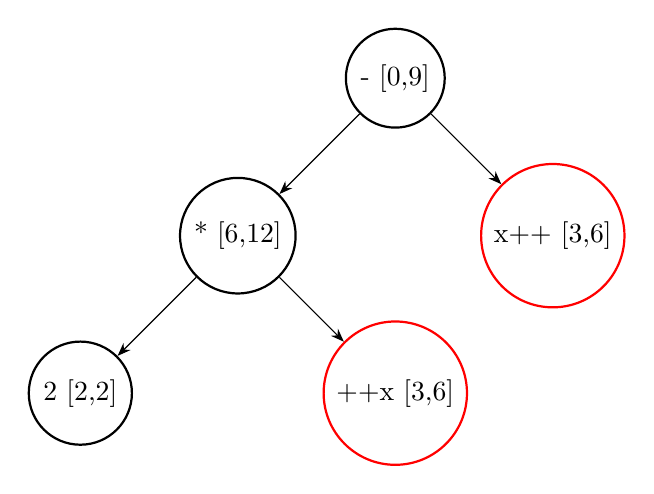
\begin{tikzpicture}

        \begin{scope}[every node/.style={circle,thick,draw}]
            \node (A) at (5,5) {- [0,9]};
            \node (B) at (3,3) {* [6,12]};
            \node (C) at (1,1) {2 [2,2]};
            \node[style={draw=red}] (D) at (5,1) {++x [3,6]};
            \node[style={draw=red}] (E) at (7,3) {x++ [3,6]};
        \end{scope}

        \begin{scope}[>={Stealth[black]}]
            \path [->] (A) edge (B);
            \path [->] (B) edge (C);
            \path [->] (B) edge (D);
            \path [->] (A) edge (E);
        \end{scope}

    \end{tikzpicture}

\end{frame}

\begin{frame}{Abstract Execution}{Boolean Expressions - Expression Tree}

    \texttt{x := \alt<5->{[3, 5]}{[2, 5]}}

    \texttt{2 * (++x) - (x++) > 5}

    ~\\\centering
    \begin{tikzpicture}

        \begin{scope}[every node/.style={circle,thick,draw}]
            \node (A) at (5,5) {- \alt<1->{[5,9]}{[0,9]}};
            \node (B) at (3,3) {* \alt<2->{[8,12]}{[6,12]}};
            \node (C) at (1,1) {2 \alt<3->{[2,2]}{[2,2]}};
            \node[style={draw=red}] (D) at (5,1) {++x \alt<5->{[4,6]}{[3,6]}};
            \node[style={draw=red}] (E) at (7,3) {x++ \alt<8->{[3,6]}{[3,6]}};
        \end{scope}

        \begin{scope}[>={Stealth[black]}]
            \path [->] (A) edge (B);
            \path [->] (B) edge (C);
            \path [->] (B) edge (D);
            \path [->] (A) edge (E);
        \end{scope}

        \begin{scope}[>={Stealth[blue]},
            every edge/.style={draw=blue}]
            \only<2->{\path [->] (A) edge[bend right=30] (B);}
            \only<3->{\path [->] (B) edge[bend right=30] (C);}
            \only<4->{\path [->] (C) edge[bend right=30] (B);}
            \only<5->{\path [->] (B) edge[bend right=30] (D);}
            \only<6->{\path [->] (D) edge[bend right=30] (B);}
            \only<7->{\path [->] (B) edge[bend right=30] (A);}
            \only<8->{\path [->] (A) edge[bend right=30] (E);}
            \only<9->{\path [->] (E) edge[bend right=30] (A);}
        \end{scope}

    \end{tikzpicture}

\end{frame}

\begin{frame}{Abstract Execution}{Boolean Expressions - \texttt{Not}}

    There are two strategies for executing the \texttt{Not} operator:
    \begin{itemize}
        \item by exploiting the De Morgan Laws and moving it towards the leaves of the boolean expression tree,\\
              e.g.: \texttt{Not(And(\textit{b1}, \textit{b2}))} $\rightarrow$ \texttt{Or(Not(\textit{b1}), Not(\textit{b2}))};
        \item by inspect the expression within and modify it in a sound way,\\
              e.g.: \texttt{Not(Eq(\textit{a1}, \textit{a2}))} $\rightarrow$ \texttt{Neq(\textit{a1}, \textit{a2})},\\
              e.g.: \texttt{Not(Not(\textit{b}))} $\rightarrow$ \texttt{\textit{b}}.
    \end{itemize}

\end{frame}

\begin{frame}{Abstract Execution}{Cahotic Iteration}

    The final task of the Abstract Interpreter is finding the invariants of each point of the program.

    In order to do so, using the Control Flow Graph, the Abstract Interpreter:
    \begin{enumerate}
        \item determines the dependencies between the invariants of different control points;
        \item put the entry point of the program in an update queue;
        \item pick the next point of the queue;
        \item calculate its invariant using the Control Flow Graph;
        \item if its invariant changed, it puts all the points that directly depends on it in the queue;
        \item if the queue is not empty, go to point 3, else finished.
    \end{enumerate}

\end{frame}

\section*{Examples}

\begin{frame}{Example with Widening}

    \begin{columns}[T]
        \begin{column}{0.4\textwidth}
            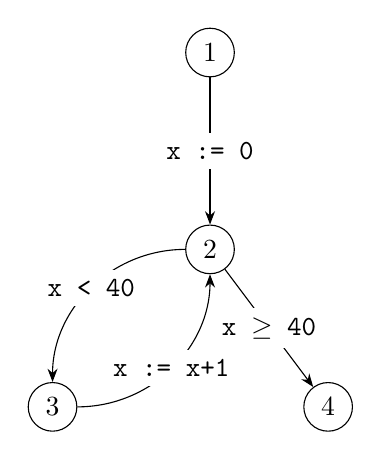
\begin{tikzpicture}
                \begin{scope}[every node/.style={circle, draw}]
                    \node (1) at (2, 4.5) {1};
                    \node (2) at (2, 2) {2};
                    \node (3) at (0, 0) {3};
                    \node (4) at (3.5, 0) {4};
                \end{scope}

                \begin{scope}[>={Stealth[black]},
                    every node/.style={fill=white}
                    ]
                    \path [->] (1) edge node{\texttt{x := 0}} (2);
                    \path [->] (2) edge[bend right=45] node{\texttt{x < 40}} (3);
                    \path [->] (2) edge node{\texttt{x $\geq$ 40}} (4);
                    \path [->] (3) edge[bend right=45] node{\texttt{x := x+1}} (2);
                \end{scope}
            \end{tikzpicture}
        \end{column}
        \begin{column}{0.4\textwidth}

            \begin{overprint}
                \onslide<1>
                Iteration: 1

                Queue: [2, 3, 4]

                \begin{itemize}
                    \item ${\cal{X}}_1 = \top^\#_{\Intmn}$
                    \item[$\nabla$] ${\cal{X}}_2 = \bot^\#_{\Intmn}$
                    \item ${\cal{X}}_3 = \bot^\#_{\Intmn}$
                    \item ${\cal{X}}_4 = \bot^\#_{\Intmn}$
                \end{itemize}

                \onslide<2>
                Iteration: 2

                Queue: [3, 4]

                \begin{itemize}
                    \item ${\cal{X}}_1 = \top^\#_{\Intmn}$
                    \item[$\nabla$] ${\cal{X}}_2 = \alert{x \in [0, 0]}$
                    \item ${\cal{X}}_3 = \bot^\#_{\Intmn}$
                    \item ${\cal{X}}_4 = \bot^\#_{\Intmn}$
                \end{itemize}

                \onslide<3>
                Iteration: 3

                Queue: [4, 2]

                \begin{itemize}
                    \item ${\cal{X}}_1 = \top^\#_{\Intmn}$
                    \item[$\nabla$] ${\cal{X}}_2 = x \in [0, 0]$
                    \item ${\cal{X}}_3 = \alert{x \in [0, 0]}$
                    \item ${\cal{X}}_4 = \bot^\#_{\Intmn}$
                \end{itemize}

                \onslide<4>
                Iteration: 4

                Queue: [2]

                \begin{itemize}
                    \item ${\cal{X}}_1 = \top^\#_{\Intmn}$
                    \item[$\nabla$] ${\cal{X}}_2 = x \in [0, 0]$
                    \item ${\cal{X}}_3 = x \in [0, 0]$
                    \item ${\cal{X}}_4 = \bot^\#_{\Intmn}$
                \end{itemize}

                \onslide<5>
                Iteration: 5

                Queue: [3, 4]

                \begin{itemize}
                    \item ${\cal{X}}_1 = \top^\#_{\Intmn}$
                    \item[$\nabla$] ${\cal{X}}_2 = x \in [0, \alert{+\inf}]$
                    \item ${\cal{X}}_3 = x \in [0, 0]$
                    \item ${\cal{X}}_4 = \bot^\#_{\Intmn}$
                \end{itemize}


                \onslide<6>
                Iteration: 6

                Queue: [4, 2]

                \begin{itemize}
                    \item ${\cal{X}}_1 = \top^\#_{\Intmn}$
                    \item[$\nabla$] ${\cal{X}}_2 = x \in [0, +\inf]$
                    \item ${\cal{X}}_3 = x \in [0, \alert{39}]$
                    \item ${\cal{X}}_4 = \bot^\#_{\Intmn}$
                \end{itemize}


                \onslide<7>
                Iteration: 7

                Queue: [2]

                \begin{itemize}
                    \item ${\cal{X}}_1 = \top^\#_{\Intmn}$
                    \item[$\nabla$] ${\cal{X}}_2 = x \in [0, +\inf]$
                    \item ${\cal{X}}_3 = x \in [0, 39]$
                    \item ${\cal{X}}_4 = \alert{x \in [40, +\inf]}$
                \end{itemize}


                \onslide<8>
                Iteration: 8

                Queue: []

                \begin{itemize}
                    \item ${\cal{X}}_1 = \top^\#_{\Intmn}$
                    \item[$\nabla$] ${\cal{X}}_2 = x \in [0, +\inf]$
                    \item ${\cal{X}}_3 = x \in [0, 39]$
                    \item ${\cal{X}}_4 = x \in [40, +\inf]$
                \end{itemize}
                Fix point


            \end{overprint}

        \end{column}
    \end{columns}

\end{frame}

\begin{frame}{Example with Narrowing}

    \begin{columns}[T]
        \begin{column}{0.4\textwidth}
            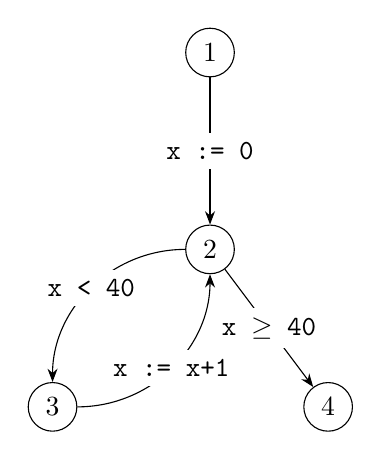
\begin{tikzpicture}
                \begin{scope}[every node/.style={circle, draw}]
                    \node (1) at (2, 4.5) {1};
                    \node (2) at (2, 2) {2};
                    \node (3) at (0, 0) {3};
                    \node (4) at (3.5, 0) {4};
                \end{scope}

                \begin{scope}[>={Stealth[black]},
                    every node/.style={fill=white}
                    ]
                    \path [->] (1) edge node{\texttt{x := 0}} (2);
                    \path [->] (2) edge[bend right=45] node{\texttt{x < 40}} (3);
                    \path [->] (2) edge node{\texttt{x $\geq$ 40}} (4);
                    \path [->] (3) edge[bend right=45] node{\texttt{x := x+1}} (2);
                \end{scope}
            \end{tikzpicture}
        \end{column}
        \begin{column}{0.5\textwidth}

            \begin{overprint}
                \onslide<1>
                Iteration: 8 + 0

                Queue: [2] $\leftarrow$ narrowing points

                \begin{itemize}
                    \item ${\cal{X}}_1 = \top^\#_{\Intmn}$
                    \item[$\Delta$] ${\cal{X}}_2 = x \in [0, +\inf]$
                    \item ${\cal{X}}_3 = x \in [0, 39]$
                    \item ${\cal{X}}_4 = x \in [40, +\inf]$
                \end{itemize}

                The narrowing begins from the previously found fix point

                \onslide<2>
                Iteration: 8 + 1

                Queue: [3, 4]

                \begin{itemize}
                    \item ${\cal{X}}_1 = \top^\#_{\Intmn}$
                    \item[$\Delta$] ${\cal{X}}_2 = x \in [0, \alert{40}]$
                    \item ${\cal{X}}_3 = x \in [0, 39]$
                    \item ${\cal{X}}_4 = x \in [40, +\inf]$
                \end{itemize}

                \onslide<3>
                Iteration: 8 + 2

                Queue: [4]

                \begin{itemize}
                    \item ${\cal{X}}_1 = \top^\#_{\Intmn}$
                    \item[$\Delta$] ${\cal{X}}_2 = x \in [0, 40]$
                    \item ${\cal{X}}_3 = x \in [0, 39]$
                    \item ${\cal{X}}_4 = x \in [40, +\inf]$
                \end{itemize}

                \onslide<4>
                Iteration: 8 + 3

                Queue: []

                \begin{itemize}
                    \item ${\cal{X}}_1 = \top^\#_{\Intmn}$
                    \item[$\Delta$] ${\cal{X}}_2 = x \in [0, 40]$
                    \item ${\cal{X}}_3 = x \in [0, 39]$
                    \item ${\cal{X}}_4 = x \in [40, \alert{40}]$
                \end{itemize}
                Fix point

                Most precise invariant


            \end{overprint}

        \end{column}
    \end{columns}

\end{frame}

\begin{frame}
    \centering \huge
    \emph{Thank you for your attention!}
\end{frame}

\end{document}